% --------------------------------------------------------------------------------

\begin{exercise}

Zeigen Sie: Die Funktion
\begin{align*}
  u(x,y) = (8\pi)^{-1}(x^2 + y^2)\ln\sqrt{x^2+y^2}, \quad (x,y) \neq (0,0)
\end{align*}
ist eine Fundamentallösung von $\Delta^2$ mit Pol in $(0,0)$ im $\R^2$, wobei
\begin{align*}
  \Delta^2u = \Delta(\Delta u) = \sum_{i,j = 1}^2 u_{x_ix_ix_jx_j}.
\end{align*}

\end{exercise}

% --------------------------------------------------------------------------------

\begin{solution}

Wir zeigen also für beliebiges $\phi \in \mathcal{D}(\R^2)$:

\begin{align*}
  \langle \Delta^2u, \phi \rangle
  :=
  \langle u, \Delta^2 \phi \rangle
  \stackrel{!}{=}
  \phi(0)
\end{align*}

Wir machen einen Ansatz wie im Skript: Sei $\Omega_\varepsilon = \R^2 \setminus \overline{B_\varepsilon(0)}$, dann soll

\begin{align*}
  \phi(0)
  \stackrel{!}{=}
  \lim_{\varepsilon \rightarrow 0}\int_{\Omega_\varepsilon} u \Delta^2 \phi dx
\end{align*}

Nun integrieren wir viermal partiell gemäß dem Satz von Gauß:

\begin{figure}[h!]
  \centering
  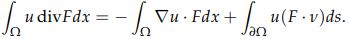
\includegraphics[width = 0.75 \textwidth]{Gauss-PI.jpg}
\end{figure}

\begin{align*}
  \int_{\Omega_\varepsilon} u \Delta^2 \phi dx
  =
  \int_{\Omega_\varepsilon} u \Div\underbrace{\nabla \Delta \phi}_F dx
  =
  -\int_{\Omega_\varepsilon} \underbrace{\nabla u}_{F} \cdot \nabla \underbrace{\Delta \phi}_{u} dx
  +
  \int_{\partial \Omega_\varepsilon} u(\nabla \Delta \phi \cdot \nu) ds
  = \\
  \int_{\Omega_\varepsilon} \underbrace{\Div\nabla u}_{\Delta u} \underbrace{\Delta \phi}_{\Div \nabla \phi} dx
  -
  \int_{\partial \Omega_\varepsilon} \Delta \phi (\nabla u \cdot \nu) ds
  +
  \int_{\partial \Omega_\varepsilon} u(\nabla \Delta \phi \cdot \nu) ds
  = \\
  -\int_{\Omega_\varepsilon} \nabla \Delta u \cdot \nabla \phi dx
  +
  \int_{\partial \Omega_\varepsilon} \Delta u (\nabla \phi \cdot \nu) ds
  -
  \int_{\partial \Omega_\varepsilon} \Delta \phi (\nabla u \cdot \nu) ds
  +
  \int_{\partial \Omega_\varepsilon} u(\nabla \Delta \phi \cdot \nu) ds
  = \\
  \underbrace{\int_{\Omega_\varepsilon} \Delta^2 u \phi dx}_{0}
  -
  \int_{\partial \Omega_\varepsilon} \phi (\nabla \Delta u \cdot \nu) ds
  +
  \int_{\partial \Omega_\varepsilon} \Delta u (\nabla \phi \cdot \nu) ds
  -
  \int_{\partial \Omega_\varepsilon} \Delta \phi (\nabla u \cdot \nu) ds
  +
  \int_{\partial \Omega_\varepsilon} u(\nabla \Delta \phi \cdot \nu) ds
\end{align*}

Die Integrale über den Rand sehen wir uns einzeln an. Dabei ist der Normalenvektor an
$\partial \Omega_\varepsilon$ gegeben durch

\begin{align*}
  \nu(x,y)
  =
  -\frac{1}{\varepsilon}
  \left(\begin{array}{c}
    x \\
    y
  \end{array}\right)
\end{align*}

Für das erste wenden wir den Mittelwertsatz der Integralrechnung an: Es existiert
ein $x_\varepsilon \in \partial B_\varepsilon(0)$, sodass

\begin{align*}
  -\int_{\partial \Omega_\varepsilon} \phi (\nabla \Delta u \cdot \nu) ds
  =
  -\int_{\partial \Omega_\varepsilon} \phi
  \Big(\frac{1}{2\pi (x^2+y^2)}
  \begin{pmatrix} x \\ y \end{pmatrix} \cdot
  - \begin{pmatrix} x \\ y \end{pmatrix}
  \frac{1}{\varepsilon}\Big) ds
  =
  \phi(x_\varepsilon) \frac{1}{2\pi \varepsilon} \int_{\partial \Omega_\varepsilon} 1 ds
  =
  \phi(x_\varepsilon)
  \stackrel{\varepsilon \rightarrow 0}{\longrightarrow}
  \phi(0)
\end{align*}

Das zweite transformieren wir in Polarkoordinaten, also $x = r\cos(\varphi), y = r\sin(\varphi)$.
Da $\Delta u = \frac{\ln(x^2 +y^2) + 2}{4 \pi}$ erhalten wir unter Anwendung der CS-Ungleichung

\begin{align*}
  |\frac{1}{4\pi} \int_{\partial \Omega_\varepsilon} (\ln(x^2 + y^2) + 2) (\nabla \phi \cdot \nu) ds|
  \leq
  \frac{\norm{\nabla \phi}}{4 \pi} (\int_0^\varepsilon \int_0^{2 \pi} \ln(r^2) r d\varphi dr) + \underbrace{\int_{\partial \Omega_\varepsilon} 2 ds}_{\stackrel{\varepsilon \rightarrow 0}{\longrightarrow 0}})
  =
  \frac{\norm{\nabla \phi}}{2} \int_0^\varepsilon \ln(r^2) r dr
  = \\
  \frac{\norm{\nabla \phi}}{2} (r^2\ln(r) - \frac{r^2}{2})\Big|_{r = 0}^\varepsilon
  =
  \norm{\nabla \phi}\frac{\varepsilon^2(2\ln(\varepsilon)-1)}{4}
  \stackrel{\varepsilon \rightarrow 0}{\longrightarrow}
  0
\end{align*}

Beim dritten berechnen wir nun zuerst $\nabla u \cdot \nu = \frac{(x^2+y^2)\ln(\sqrt{x^2+y^2})}{4\pi}+\frac{x^2+y^2}{8\pi}$.
Dann erhalten wir wiederum mit TRAFO:

\begin{align*}
  |\int_{\partial \Omega_\varepsilon} \Delta \phi (\nabla u \cdot \nu) ds|
  \leq
  \norm{\phi}  \int_0^\varepsilon \int_0^{2 \pi} \frac{r^4\ln{r}}{4\pi} + \frac{r}{8\pi} d\varphi dr
  =
  \norm{\phi} \int_0^\varepsilon \frac{r^4\ln{r}}{2} + \frac{r}{4} dr
  =
  \norm{\phi}(\frac{5\varepsilon^5 \ln{\varepsilon} - \varepsilon^5}{50} + \frac{\varepsilon^2}{8})
  \stackrel{\varepsilon \rightarrow 0}{\longrightarrow}
  0
\end{align*}
Auch beim letzten können wir das so durchführen:

\begin{align*}
  |\frac{1}{8\pi} \int_{\partial \Omega_\varepsilon} (x^2 + y^2)(\ln(\sqrt{x^2 + y^2})) (\nabla \Delta \phi \cdot \nu) ds|
  \leq
  \frac{\norm{\nabla \Delta \phi}}{8 \pi} \int_0^\varepsilon \int_0^{2 \pi} r^3 \ln(r) d\varphi dr
  =
  \frac{\norm{\nabla \Delta \phi}}{4} \int_0^\varepsilon r^3 \ln(r) dr
  =\\
  \frac{\norm{\nabla \Delta \phi}}{4} \frac{4 \varepsilon^4 \ln(\varepsilon) - \varepsilon^4 }{16}
  \stackrel{\varepsilon \rightarrow 0}{\longrightarrow}
  0
\end{align*}

Damit ist diese Funktion also wirklich eine Fundamentallösung.

\textbf{Alternative Lösung:}

Durch elementares Ableiten erhält man
\begin{align}
    (\Delta u)(x, y) = \frac{\log(\sqrt{x^2 + y^2}) + 1}{2 \pi}.
\end{align}
Nach Satz 4.1 ist $\frac{\log(r)}{2 \pi}$ eine Fundamentallösung des Laplace-Operators, wobei $r = \sqrt{x^2 + y^2}$. Daher gilt
\begin{align}
    \left\langle \Delta^2 u, \phi \right\rangle =  \left\langle \Delta \left( \frac{\log(\sqrt{x^2 + y^2}) + 1}{2 \pi}\right), \phi \right\rangle
    = \\ \left\langle \Delta \left( \frac{\log(\sqrt{x^2 + y^2})}{2 \pi}\right) + \underbrace{\Delta \frac{1}{2 \pi}}_{= 0}, \phi \right\rangle =
    \left\langle \Delta \frac{\log(r)}{2 \pi}, \phi \right\rangle \stackrel{\text{Satz 4.1}}= \langle \delta_0, \phi \rangle.
\end{align}
\end{solution}

% --------------------------------------------------------------------------------
